\chapter{Testrig}
\section{Introduction}
When designing a complex system sych as a hybrid vehicle, being continuously be
able to test the system is important to validate that the requirements are met
and to verify the models. To be able to do a full system test, the car has to be
physically run on a track. This can be cumbersome, or in the case of the London
track, impossible at times. Therefore, a test rig is designed and built. The
design process uses the V-model approach with a set of live requirements and
continuous unit and integration testing. The overall goal is to not only be able
to do a faithful simulation of the EcoCar track in London, but to be able to
supply any track (with certain limitations on power and speed demands) to the
test rig and simulations on the car.

\section{Requirements}
The requirements on the test rig are designed to capture the essential demands
on the system. Firstly, the high level User requirements are set. The user goals
of the test rig are set from a viewpoint of how the testrig would be used in the
SEM 2016 in London. This means that the power and speed goals are set to fit the
London track and that the physical appearance of the test rig should fit Elba.

\section{Temp notes}
Modeled negative forces acting on vehicle (gravity, air resistance, friction): 
Torque required on wheel of ELBA:$$T_r = F_r\*r_w$$
Torque required for vals on test rig: $$T_t = \frac{T_r\*r_t}{r_w}$$
Required torque for motor, $T_m$:
$$T_m = T_t + J\ddot{\phi} + d\dot{\phi} + k\phi$$


\begin{figure}[H]
    \centering
    \label{fig:testrig_power_required_motor}
    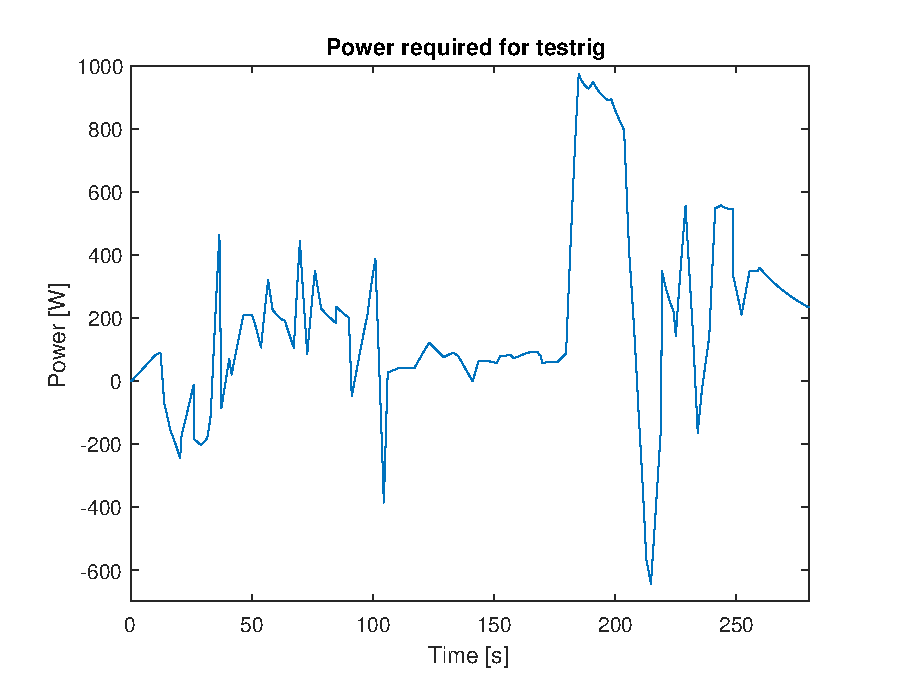
\includegraphics[width=0.5\textwidth]{./testrig/power_required_testrig.eps}
    \caption{Power required for the motor on the testrig.}
\end{figure}
